\chapter{Experimentos \& Análises}
\label{cap6}



A partir dos dados coletados, foi realizada uma análise dos dados seguindo os critérios levantados durante a proposta do atual trabalho.
%
Tal análise visa compreender o consumo de recurso usado pelas arquiteturas com base em suas características específicas.



Cada caso de análise é dividido em experimentos, na qual cada experimento tem o objetivo de analisar um conjunto de recursos dado alguma situação.
%
Nesse sentido, faz sentido agrupar tais experimentos, agrupados na Seção~\ref{sec:experimentos}, para posterior comparação.



%ccm todo gráfico precisa responder a alguma pergunta.
% 1- Formular a pergunta com base no que definiu no Cap.4
% 2- quem está envolvido, quais são os parâmetros, quais são constantes
% 3- Descrever o perfil/modus operandi do experimento
% 4- Mostra a figura
% 5- Analisa os resultados com base na expectativa no Cap.4 (foi similar, diferente, por quê?)
% 6 - Precisa manter em mente que as figuras devem manter uma escala para poder comparar entre diferentes arquiteturas


\section{Experimentos}
\label{sec:experimentos}



Cada experimento utiliza as arquiteturas de microsserviços para jogos \ac{mmorpg} Rudy, Salz e Willson.
%
Cada arquitetura é executada no mesmo ambiente, isolados por momentos diferentes.
%
Para cada arquitetura, é realizado três execuções com os mesmos parâmetros.
%
Em cada execução, o seguinte protocolo é seguido:


\begin{enumerate}
 \item Início dos serviços do banco de dados.
 \item Início dos serviços de jogo.
 \item Início dos clientes.
 \item Clientes são escalados de 1 em 1 até 100, com 30 segundos de intervalo.
 \item Todos os serviços em todos os ambientes são removidos, mantendo somente os dados capturados.
\end{enumerate}


A partir de tais execuções, os dados são capturados, processados e analisados.
%
Durante as execuções, os dados sobre a latência da rede mostraram-se estáveis, variando entre 5ms e 15ms, dessa forma foram ignorados como um experimento a parte, porém serviram para validar a estabilidade da rede.



\subsection{Consumo de \ac{cpu}}



Este experimento visa analisar o consumo de \ac{cpu} unitariamente, em relação ao número de jogadores simultâneos.
%
Espera-se que o seu crescimento seja de tendência linear junto ao crescimento de jogadores concorrentes.
%
Neste contexto existem os seguintes valores:



\begin{itemize}
    \item Jogadores simultâneos: Variável capturada a partir do microsserviço de jogo.
    \item Consumo de \ac{cpu}: Variável capturada a partir do monitor de recursos do Docker.
\end{itemize}

Nota-se que o número de jogadores simultâneos e o consumo de \ac{cpu} são indexados pelo tempo a qual tais dados foram capturados.
%
Nesse sentido podemos relacionar o número de jogadores simultâneos ao consumo de \ac{cpu} dos microsserviços e do banco de dados.
%
Dado tal contexto, faz sentido realizar uma análise separando os ambientes de Banco de Dados de Microsserviços.

\subsubsection{Banco de Dados}



Considerando o ambiente de banco de dados, podemos realizar a associação de número de jogadores simultâneos e \ac{cpu} consumida pelos contêineres de banco de dados.
%
Essa associação é realizada pelo tempo de registro das métricas.
%
O resultado desta associação pode ser visualizado na Figura~\ref{fig:experimento_db_cpu}.



\begin{figure}[htb!]
    \caption{Consumo de \ac{cpu} dos bancos de dados}
    \label{fig:experimento_db_cpu}

    \begin{subfigure}{0.5\textwidth}
        \centering
        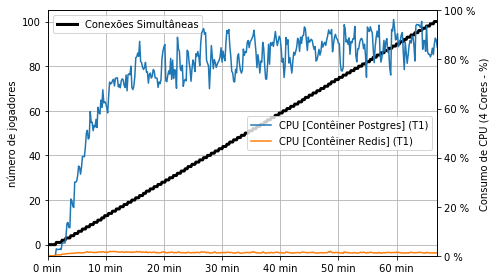
\includegraphics[width=.95\linewidth]{figuras/testes/r_cpu_db.png}
        \caption{Bancos de Dados da arquitetura Rudy}
        \label{fig:r_cpu_db}
    \end{subfigure}%
    \begin{subfigure}{0.5\textwidth}
        \centering
        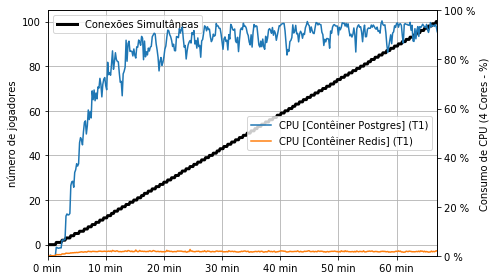
\includegraphics[width=.95\linewidth]{figuras/testes/s_cpu_db.png}
        \caption{Bancos de Dados da arquitetura Salz}
        \label{fig:s_cpu_db}
    \end{subfigure}\\

    \begin{subfigure}{0.5\textwidth}
        \centering
        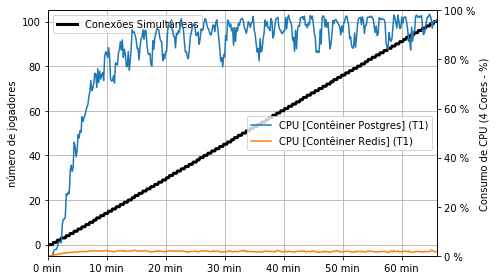
\includegraphics[width=.95\linewidth]{figuras/testes/w_cpu_db.png}
        \caption{Bancos de Dados da arquitetura Willson}
        \label{fig:w_cpu_db}
    \end{subfigure}

    Fonte: O próprio autor.
\end{figure}


A Figura~\ref{fig:experimento_db_cpu} exibe o comportamento do consumo de \ac{cpu} durante a execução dos testes para as arquiteturas Rudy (Subfigura~\ref{fig:r_cpu_db}), Salz (Subfigura~\ref{fig:s_cpu_db}) e Willson (Subfigura~\ref{fig:w_cpu_db}).
%
Em todas as figuras é notório o seguinte comportamento:

\begin{itemize}
 \item Baixo consumo de \ac{cpu} do servidor de dados temporários (Redis), com comportamento linear estável.
 \item Alto consumo de \ac{cpu} do servidor de dados permanentes (PostgreSQL), com comportamento multimodal.
\end{itemize}

Este comportamento era esperado, dado a natureza distinta de ambos os banco de dados, na qual PostgreSQL é um banco de dados \ac{acid} e o Redis é um banco de dados \ac{nosql}.
%
Entretanto é notório a discrepância entre ambos os bancos de dados, afimando-se que o banco de dados temporário é estável em relação ao consumo de \ac{cpu}.

Ao analisar o comportamento do banco de dados persistentes para as arquiteturas Rudy (Subfigura~\ref{fig:r_cpu_db}), Salz (Subfigura~\ref{fig:s_cpu_db}) e Willson (Subfigura~\ref{fig:w_cpu_db}) observamos um comportamento diferente na arquitetura Rudy.
%
Dada esta percepção, faz sentido analisar a tendência destas curvas com base em sua média.
%
Nesse sentido, a Tabela~\ref{tab:cpu_db_media_quadrantes} exibe os valores das médias baseado em todo o decorrer do experimento e dividindo o experimento em quadrantes.

\begin{table}[htb!]
\centering
\begin{adjustbox}{max width=\textwidth}
\caption{Consumo de \ac{cpu} por quadrante pelo PostgreSQL.}
\label{tab:cpu_db_media_quadrantes}
\begin{tabular}{l|l|l|l}

\hline \hline

Quadrante & Rudy    & Salz    & Willson \\ \hline \hline

Primeiro  & 50.60\% & 53.10\% & 58.15\% \\ \hline

Segundo   & 80.66\% & 88.04\% & 89.86\% \\ \hline

Terceiro  & 85.61\% & 90.77\% & 92.50\% \\ \hline

Quarto    & 86.94\% & 92.07\% & 93.48\% \\ \hline \hline

\end{tabular}

\end{adjustbox}

Fonte: O próprio autor.
\end{table}

Torna-se visível a diferença do consumo de \ac{cpu} entre as arquiteturas pelo banco de dados.
%
A partir destes dados podemos deduzir que:

\begin{itemize}
 \item Arquitetura Rudy consome menos \ac{cpu} do banco de dados persistentes; e \item Arquitetura Salz e Willson consomem \ac{cpu} na mesma proporsão, com a arquitetura Salz tendo uma leva tendência a consumir menos \ac{cpu}.
\end{itemize}

Para tornar esta diferença visível ao longo de toda a progressão da carga, faz sentido exibir esta informação em um gráfico de linha.
%
A Figura~\ref{fig:cpu_db_media_por_jogador} exibe a média de consumo de \ac{cpu} pelo contêiner PostgreSQL comparado ao número de jogadores simultâneos.

\begin{figure}[htb!]
  \caption{Consumo de \ac{cpu} pelo PostgreSQL comparado ao número de jogadores simultâneos.}
  \label{fig:cpu_db_media_por_jogador}
  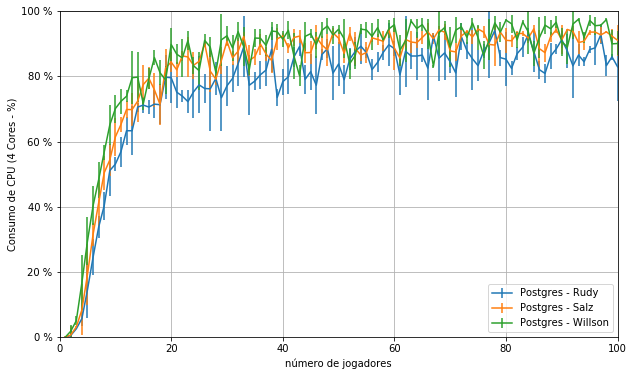
\includegraphics[width=0.8\textwidth]{figuras/analise/cpu_db_media_por_jogador.png}
  \centering

  Fonte: O próprio autor.
\end{figure}

Conforme exibido na Figura~\ref{fig:cpu_db_media_por_jogador}, pode-se deduzir que em todo caso as arquiteturas Rudy, Salz e Willson seguem a seguinte expressão:

$$
    CPU(db\_postgresql_{r}) < CPU(db\_postgresql_{s}) \approx CPU(db\_postgresql_{w})
$$

O banco de dados temporários consome pouca \ac{cpu}, comparado ao banco de dados persistentes.
%
Entretanto, faz sentido realizar a mesma análise para validar se existe alguma diferença no seu uso conforme a arquitetura empregada.
%
Dessa forma foi dividido em quadrantes para analisar o consumo médio de \ac{cpu}, a qual é exibido na Tabela~\ref{tab:cpu_redis_media_quadrantes}.

\begin{table}[htb!]
\centering
\begin{adjustbox}{max width=\textwidth}
\caption{Consumo de \ac{cpu} por quadrante pelo Redis.}
\label{tab:cpu_redis_media_quadrantes}
\begin{tabular}{|l|l|l|l|}

\hline

Quadrante & Rudy    & Salz    & Willson \\ \hline

Primeiro  & 1.24\% & 1.46\% & 1.60\% \\ \hline

Segundo   & 1.32\% & 1.79\% & 1.81\% \\ \hline

Terceiro  & 1.28\% & 1.75\% & 1.75\% \\ \hline

Quarto    & 1.26\% & 1.73\% & 1.72\% \\ \hline

\end{tabular}

\end{adjustbox}

Fonte: O próprio autor.
\end{table}

Dado os valores da Tabela~\ref{tab:cpu_redis_media_quadrantes}, pode-se obter as seguintes conclusões:

\begin{itemize}
 \item Rudy consome menos \ac{cpu} do banco de dados temporários; e
 \item A arquitetura Salz e Willson consomem \ac{cpu} com o mesmo comportamento.
\end{itemize}

Para tornar esta diferença visível ao longo de toda a progressão da carga, faz sentido exibir esta informação em um gráfico de linha.
%
A Figura~\ref{fig:cpu_redis_media_por_jogador} exibe um gráfico a qual compara a média de consumo de \ac{cpu} conforme o número de jogadores simultâneos.

\begin{figure}[htb!]
  \caption{Consumo de \ac{cpu} pelo PostgreSQL comparado ao número de jogadores simultâneos.}
  \label{fig:cpu_redis_media_por_jogador}
  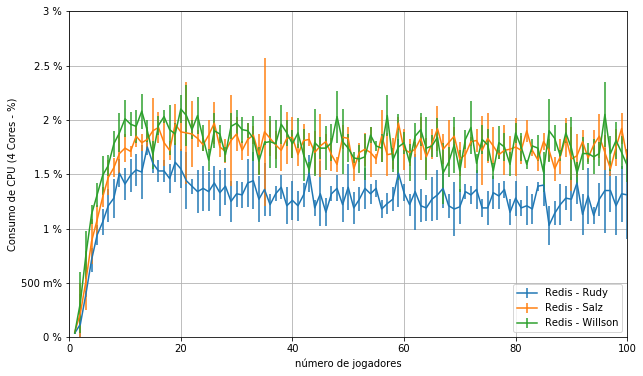
\includegraphics[width=0.8\textwidth]{figuras/analise/cpu_redis_media_por_jogador.png}
  \centering

  Fonte: O próprio autor.
\end{figure}

Conforme exibido na Figura~\ref{fig:cpu_redis_media_por_jogador}, podemos deduzir que em todo caso as arquiteturas Rudy, Salz e Willson seguem a seguinte expressão:

$$
    CPU(db\_redis_{r}) < CPU(db\_redis_{s}) \approx CPU(db\_redis_{w})
$$

%ccm Precisa fazer uma legenda das letrinhas. Pode ser parágrafo ou itemize.
Nota-se que o consumo de recurso do banco de dados temporários e banco de dados persistentes exibiram o mesmo comportamento.
%
Dessa forma, podemos generalizar o comportamento do consumo de \ac{cpu} das arquiteturas Rudy, Salz e Willson para banco de Dados:

$$
    CPU(db_{r}) < CPU(db_{s}) \approx CPU(db_{w})
$$

Este comportamento é dado pela característica do microsserviço \textit{rcrud} que realiza uma multiplexação de conexões entre o banco de dados e a arquitetura.
%
Entretanto, esta característica pode ser por dois motivos:

\begin{itemize}
 \item O banco de dados está otimizado para responder uma única conexão, consumindo menos \ac{cpu}; ou
 \item O banco de dados não consome tanta \ac{cpu} por ter um microsserviço que tornou-se um gargalo como frente do banco de dados.
\end{itemize}

Dado estas duas hipóteses, faz sentido mensurar a qualidade de serviço entregue ao usuário.
%
Podemos mensurar qual das hipóteses é mais valiosa para a qualidade de serviço com base no tempo de resposta do usuário.


\subsubsection{Microsserviços}

Considerando o ambiente de banco de dados, podemos realizar a associação de número de jogadores simultâneos e \ac{cpu} consumida pelos contêineres de banco de dados.
%
Essa associação é realizada pelo tempo de registro das métricas.
%
O resultado desta associação pode ser visualizado na Figura~\ref{fig:experimento_game_cpu}.

\begin{figure}[htb!]
    \caption{Consumo de \ac{cpu} dos microsserviços}
    \label{fig:experimento_game_cpu}

    \begin{subfigure}{0.5\textwidth}
        \centering
        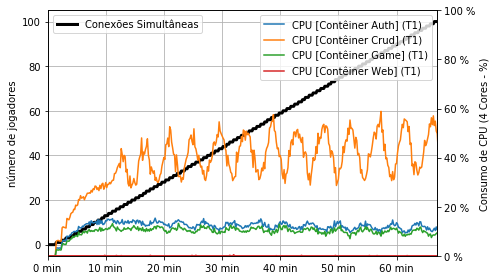
\includegraphics[width=.95\linewidth]{figuras/testes/r_cpu_game.png}
        \caption{Microsserviços da arquitetura Rudy}
        \label{fig:r_cpu_game}
    \end{subfigure}%
    \begin{subfigure}{0.5\textwidth}
        \centering
        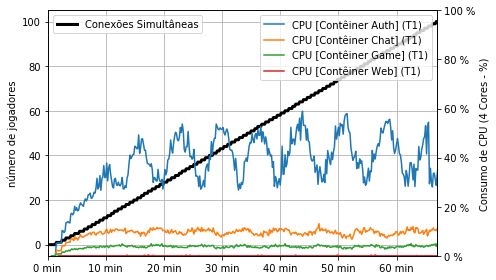
\includegraphics[width=.95\linewidth]{figuras/testes/s_cpu_game.png}
        \caption{Microsserviços da arquitetura Salz}
        \label{fig:s_cpu_game}
    \end{subfigure}

    \begin{subfigure}{0.5\textwidth}
        \centering
        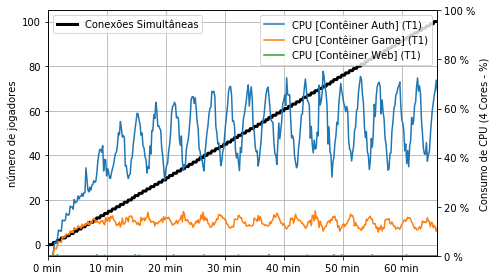
\includegraphics[width=.95\linewidth]{figuras/testes/w_cpu_game.png}
        \caption{Microsserviços da arquitetura Willson}
        \label{fig:w_cpu_game}
    \end{subfigure}%

    Fonte: O próprio autor.
\end{figure}

Conforme exibido nas Figuras~\ref{fig:r_cpu_game}, ~\ref{fig:s_cpu_game} e ~\ref{fig:w_cpu_game}, podemos observar as seguintes características:

\begin{itemize}
 \item Os microsserviços \textit{rweb}, \textit{sweb} e \textit{wweb} consomem pouca \ac{cpu} comparado a todos os outros microsserviços das arquiteturas;
 \item Os microsserviços \textit{rcrud}, \textit{sauth} e \textit{wauth} são os microsserviços que mais consomem \ac{cpu} nas arquiteturas Rudy, Salz e Willson;
\end{itemize}

Faz sentido analisar a média do consumo de \ac{cpu} dos microsserviços dividindo em quadrantes.
%
Dessa forma, podemos obter dados significantes para realizar comparações a partir destes dados.
%
A Tabela~\ref{tab:cpu_microsservicos_media_quadrantes} exibe a média de consumo de \ac{cpu} por quadrante de todos os microsserviços.

\begin{table}[htb!]
\centering
\begin{adjustbox}{max width=\textwidth}
\caption{Consumo de \ac{cpu} por quadrante dos microsserviços.}
\label{tab:cpu_microsservicos_media_quadrantes}

\begin{tabular}{|l|l|l|l|l|}
\hline
Microsserviço & Primeiro Quadrante & Segundo Quadrante & Terceiro Quadrante & Quarto Quadrante \\ \hline
rauth         & 11.22\%            & 12.52\%           & 11.88\%            & 11.56\%          \\ \hline
rcrud         & 25.97\%            & 41.83\%           & 42.5\%             & 43.62\%          \\ \hline
rgame         & 8.92\%             & 10.54\%           & 10.14\%            & 9.58\%           \\ \hline
rweb          & 0.01\%             & 0.01\%            & 0.01\%             & 0.01\%           \\ \hline
sauth         & 26.08\%            & 39.95\%           & 43.22\%            & 40.96\%          \\ \hline
schat         & 8.34\%             & 9.97\%            & 9.59\%             & 9.61\%           \\ \hline
sgame         & 3.12\%             & 3.87\%            & 3.72\%             & 3.85\%           \\ \hline
sweb          & 0.01\%             & 0.01\%            & 0.01\%             & 0.01\%           \\ \hline
wauth         & 23.79\%            & 50.73\%           & 57.11\%            & 56.69\%          \\ \hline
wgame         & 9.68\%             & 14.20\%           & 13.66\%            & 13.42\%          \\ \hline
wweb          & 0.01\%             & 0.01\%            & 0.01\%             & 0.01\%           \\ \hline
\end{tabular}
\end{adjustbox}

Fonte: O próprio autor.
\end{table}

A Tabela~\ref{tab:cpu_microsservicos_media_quadrantes} mostra o crescimento do consumo de carga médio dos quadrantes.
%
Estes dados são importantes, haja vista que os mesmos permitem analisar o comportamento das curvas removendo oscilações notórias na visualização do consumo de \ac{cpu}.
%
A partir desta tabela podemos realizar as seguintes conclusões:

\begin{itemize}
 \item Entre os microsserviços \textit{rcrud}, \textit{sauth} e \textit{wauth}, o com maior consumo é o microsserviço \textit{wauth}.
 \item Os microsserviços \textit{rweb}, \textit{sweb} e \textit{wweb} possuem o mesmo consumo, em média.
\end{itemize}

Faz sentido, a partir destas conclusões, analisar a média em relação a progressão de usuários.
%
A visualização da média de consumo de \ac{cpu} por usuário simultâneo tem como objetivo remover ruídos que possam afetar a visualização dos dados.

\begin{figure}[htb!]
    \caption{Média do consumo de \ac{cpu} dos microsserviços por jogador simultâneo}
    \label{fig:cpu_game_media_por_jogador}

    \begin{subfigure}{0.5\textwidth}
        \centering
        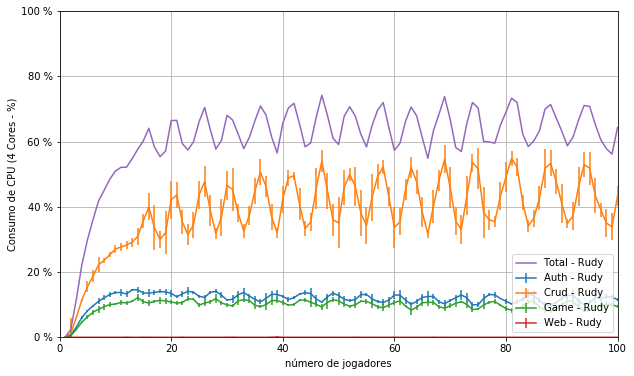
\includegraphics[width=.95\linewidth]{figuras/analise/cpu_r_arch_media_por_jogador.png}
        \caption{Microsserviços da arquitetura Rudy}
        \label{fig:cpu_r_arch_media_por_jogador}
    \end{subfigure}%
    \begin{subfigure}{0.5\textwidth}
        \centering
        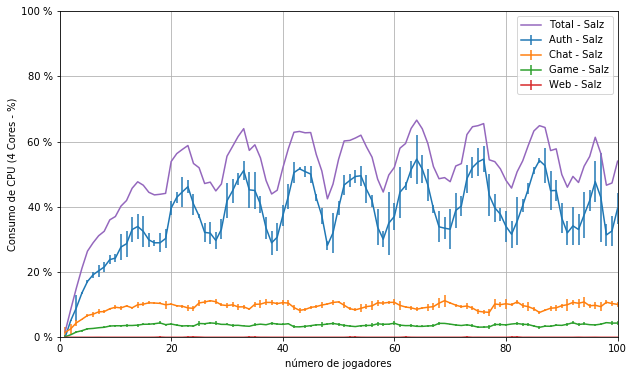
\includegraphics[width=.95\linewidth]{figuras/analise/cpu_s_arch_media_por_jogador.png}
        \caption{Microsserviços da arquitetura Salz}
        \label{fig:cpu_s_arch_media_por_jogador}
    \end{subfigure}

    \begin{subfigure}{0.5\textwidth}
        \centering
        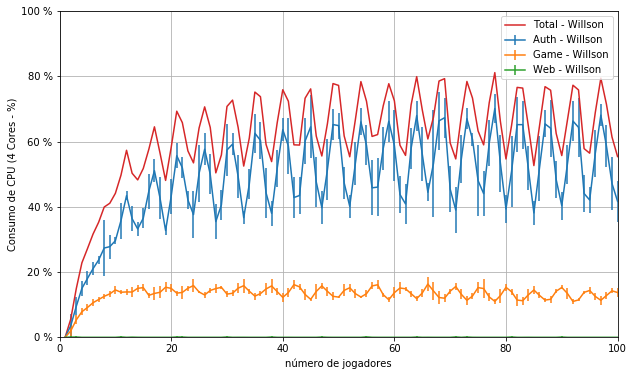
\includegraphics[width=.95\linewidth]{figuras/analise/cpu_w_arch_media_por_jogador.png}
        \caption{Microsserviços da arquitetura Willson}
        \label{fig:cpu_w_arch_media_por_jogador}
    \end{subfigure}%

    Fonte: O próprio autor.
\end{figure}

A Figura~\ref{fig:cpu_game_media_por_jogador} tem como objetivo exibir a média de consumo de \ac{cpu} por jogador, assim permitindo analisar o comportamento das curvas.
%
Entretanto, nota-se que todos os microsserviços contém uma característica senoidal, onde sua amplitude aumenta com a quantidade de jogadores, na qual já era visível na Figura~\ref{fig:experimento_game_cpu}.
%
Entretanto, neste gráfico também é visível o erro de cada média.
%
Este erro é dado pela variância do conjunto de dados obtidos na determinada faixa de jogadores simultâneos.
%
Ter um valor de variância alto significa que, por mais que a média seja um bom valor para a métrica, diversos pontos da mesma faixa estão longe deste valor.
%
Dessa forma, podemos interpretar como um erro, neste contexto.

Podemos deduzir as seguintes características a partir da Figura~\ref{fig:cpu_game_media_por_jogador}:

\begin{itemize}
 \item Os microsserviços que contém maior erro são os que estão relacionados a acesso de dados para autenticação ou/e geração de assinaturas de dados para outros serviços (\textit{rcrud, sauth e wauth});
 \item Os microsserviços que contém maior erro, são os que lideram a lista de maior consumo de \ac{cpu}, porém nota-se a partir dos demais microsserviços que esta relação não é proporcional a carga; e
 \item O valor total de consumo de \ac{cpu} mudou conforme a arquitetura.
\end{itemize}

Dado o último critério, utilizando a curva de total consumido das Sub figuras~\ref{fig:cpu_r_arch_media_por_jogador}, ~\ref{fig:cpu_s_arch_media_por_jogador} e ~\ref{fig:cpu_w_arch_media_por_jogador},  podemos comparar o total de consumo de \ac{cpu} por cada arquitetura.
%
A Tabela~\ref{tab:consumo_total_cpu} exibe os valores baseados em quadrantes, para realizar a comparação com valores.


\begin{table}[htb!]
\centering
\begin{adjustbox}{max width=\textwidth}
\caption{Consumo total de \ac{cpu} por quadrante dos microsserviços.}
\label{tab:consumo_total_cpu}

\begin{tabular}{|l|l|l|l|l|}
\hline
Arquitetura & Primeiro Quadrante & Segundo Quadrante & Terceiro Quadrante & Quarto Quadrante \\ \hline
Rudy        & 47.05\%            & 64.51\%           & 65.25\%            & 64.31\%          \\ \hline
Salz        & 38.74\%            & 53.87\%           & 56.74\%            & 54.27\%          \\ \hline
Willson     & 44.60\%            & 65.76\%           & 67.94\%            & 66.98\%          \\ \hline
\end{tabular}
\end{adjustbox}

Fonte: O próprio autor.
\end{table}

A partir dos dados da Tabela~\ref{tab:consumo_total_cpu}, podemos referenciar que a arquitetura Salz consome menos \ac{cpu} que a arquitetura Rudy e Willson.
%
Faz sentido realizar a visualização das três curvas de totais em um único gráfico a fim de exibir esta relação.
%
A Figura~\ref{fig:consumo_total_cpu} exibe esta comparação.

\begin{figure}[htb!]
  \caption{Comparação de consumo total de \ac{cpu} pelas arquiteturas.}
  \label{fig:consumo_total_cpu}
  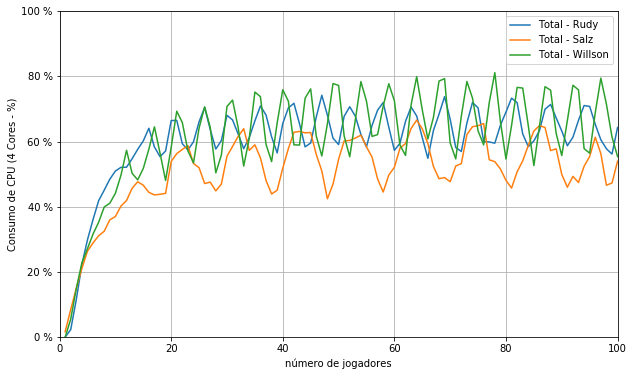
\includegraphics[width=0.8\textwidth]{figuras/analise/cpu_total_archs.png}
  \centering

  Fonte: O próprio autor.
\end{figure}

Dado a Figura~\ref{fig:consumo_total_cpu} e a Tabela~\ref{tab:consumo_total_cpu}, podemos afirmar que:

$$
    CPU(microsservicos_{s}) < CPU(microsservicos_{r}) < CPU(microsservicos_{w})
$$

Torna-se notório que tal sequência respeita a ordem de interconexões dos microsserviços.
%
Nesse sentido, a arquitetura Salz possui mais conexões que a arquitetura Rudy, que possui mais conexões que a arquitetura Willson.

Nota-se que possuir um consumo de \ac{cpu} maior que outra arquitetura não implica em ser uma arquitetura melhor.
%
Podemos encontrar dois casos para um consumo de \ac{cpu} ao comparar duas arquiteturas:

\begin{itemize}
 \item A arquitetura possui pouca carga para estressar a \ac{cpu}; ou
 \item A arquitetura converge para tal valor, visto que está com gargalo em outro recurso necessário;
\end{itemize}

Para o caso desta análise, podemos descartar a primeira alternativa.
%
Para este caso podemos analisar que a curva estabiliza o seu crescimento entre 20 e 40 jogadores simultâneos, a mesma faixa onde os bancos de dados estabilizaram seu crescimento (visível na Figura~\ref{fig:cpu_db_media_por_jogador}).
%
Dessa forma pode-se justificar o aumento de erros nas médias nos microsserviços com acesso ao banco conforme o aumento da carga no serviço.

Outra característica das curvas obtidas é a frequência da senoide encontrada, característica visível na Figura~\ref{fig:consumo_total_cpu}.
%
Nota-se que a frequência é escalada tal qual a crista de uma onda entra em contato com o vale da outra onda.
%
Tal característica das curvas não é coincidência, sendo resultado do escalonador de contêineres.
%
A Figura~\ref{fig:cpu_w_arch_media_por_jogador} é a que melhor exemplifica este comportamento, haja vista que a arquitetura Willson possui somente dois microsserviços que são impactados diretamente por este escalonador.


\subsection{Consumo de Memória}



Este experimento visa analisar o consumo de memória unitariamente, em relação ao número de jogadores simultâneos.
%
Espera-se que o seu crescimento seja linear seguindo o crescimento de jogadores concorrentes.
%
Neste contexto existem os seguintes valores:



\begin{itemize}
    \item Jogadores simultâneos: Variável capturada a partir do microsserviço de jogo.
    \item Consumo de memória: Variável capturada a partir do monitor de recursos do Docker.
\end{itemize}

Nota-se que o número de jogadores simultâneos e o consumo de memória são indexados pelo tempo a qual tais dados foram capturados.
%
Nesse sentido podemos relacionar o número de jogadores simultâneos ao consumo de memória dos microsserviços e do banco de dados.
%
Dado tal contexto, faz sentido realizar uma análise separando os ambientes de Banco de Dados de Microsserviços.

\subsubsection{Banco de Dados}



Considerando o ambiente de banco de dados, podemos realizar a associação de número de jogadores simultâneos e memória consumida pelos contêineres de banco de dados.
%
Essa associação é realizada pelo tempo de registro das métricas.
%
O resultado desta associação pode ser visualizado na Figura~\ref{fig:experimento_db_mem}.



\begin{figure}[htb!]
    \caption{Consumo de memória dos bancos de dados}
    \label{fig:experimento_db_mem}

    \begin{subfigure}{0.5\textwidth}
        \centering
        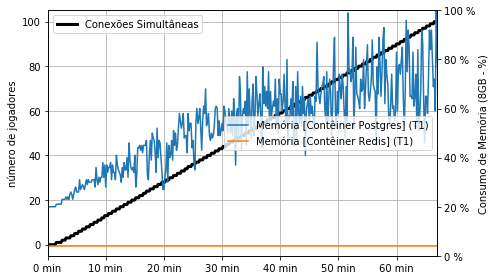
\includegraphics[width=.95\linewidth]{figuras/testes/r_mem_db.png}
        \caption{Bancos de Dados da arquitetura Rudy}
        \label{fig:r_mem_db}
    \end{subfigure}%
    \begin{subfigure}{0.5\textwidth}
        \centering
        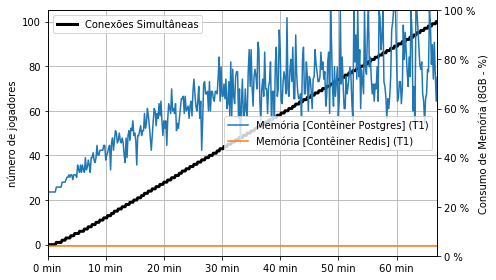
\includegraphics[width=.95\linewidth]{figuras/testes/s_mem_db.png}
        \caption{Bancos de Dados da arquitetura Salz}
        \label{fig:s_mem_db}
    \end{subfigure}\\

    \begin{subfigure}{0.5\textwidth}
        \centering
        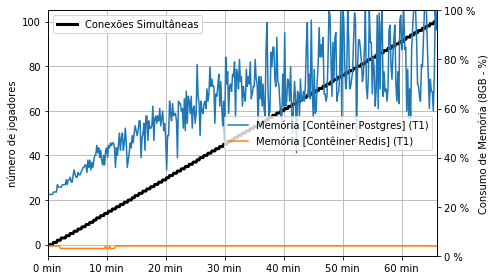
\includegraphics[width=.95\linewidth]{figuras/testes/w_mem_db.png}
        \caption{Bancos de Dados da arquitetura Willson}
        \label{fig:w_mem_db}
    \end{subfigure}

    Fonte: O próprio autor.
\end{figure}

Percebe-se, a partir da Figura~\ref{fig:experimento_db_mem}, que o banco com maior estresse é o PostgreSQL.
%
O banco de dados Redis consome uma quantidade de memória visivelmente fixa.
%
Entretanto o banco de dados Redis é utilizado para armazenamento de dados da sessão do cliente em memória.
%
Dessa forma, faz sentido calcular a quantidade de memória consumida por cada usuário para garantir que na totalidade este valor não é significativo em porcentagem.

Para realizar a autenticação é utilizado \ac{jwt}.
%
Entretanto é necessário garantir uma única conexão por usuário.
%
A unicidade é realizada utilizando o Redis, armazenando uma sequência de caracteres aleatórias em um campo formatado com o nome do usuário.
%
O trecho de código que realiza esta operação é exibido na Figura~\ref{lst:seq_chars_redis}.



\begin{lstlisting}[language=go,firstnumber=1, caption={Informações do Bloco},label={lst:seq_chars_redis}]
package merepositories

// mmosandbox/infra/merepositories/token_repositoriy.go

// GenerateToken based in username from account
func (repository *TokenRepository) GenerateToken(username string) string {
    token := repository.randomToken()
    repository.set(repository.keyPattern(username), token)

    return token
}

// keyPattern to store into redis
func (repository *TokenRepository) keyPattern(username string) string {
    return fmt.Sprintf("session.%s", username)
}

// randomToken with 256 runes
func (repository *TokenRepository) randomToken() string {
    return randomize.RandStringRunes(256)
}
\end{lstlisting}

O repositório de dados \textit{TokenRepository}\footnote{\textit{TokenRepository}: \url{https://github.com/schweigert/mmosandbox/blob/master/infra/merepositories/token_repositoriy.go}} contém as operações exibidas na Listagem~\ref{lst:seq_chars_redis}.
%
Este repositório gera a chave com o padrão \textit{session.\%s} e uma sequência de caracteres aleatória de 256 bytes.

Para realizar este calculo é necessário estimar o custo de armazenamento das chaves.
%
Por padrão, os clientes de ataque geram nomes de usuários de 32 caracteres.
%
Com tais dados, podemos estimar o custo de memória por usuário.
%
Pode-se calcular o consumo de memória por um único jogador simultâneo utilizando a seguinte fórmula:

\begin{multline}
m_j = m_{chave} + m_{padrao} + m_{valor} \\
\Rightarrow m_j = 32bytes + 8bytes + 256bytes = 296bytes
\end{multline}

Logo, ao ter 100 jogadores simultâneos, o serviço Redis consumirá aproximadamente 29Kb para armazenamento de memória.
%
Tal valor é insignificante comparado ao total de memória disponível no hospedeiro, dessa forma exibindo um comportamento retilínio na Figura~\ref{fig:experimento_db_mem}.

Entretanto o PostgreSQL exibe um crescimento linear visivel na Figura~\ref{fig:experimento_db_mem}.
%
Faz sentido sanitizar estas curvas com a média dos quadrantes.
%
A Tabela~\ref{tab:mem_db_media_quadrantes} exibe o consumo de memória médio por quadrante.

\begin{table}[htb!]
\centering
\begin{adjustbox}{max width=\textwidth}
\caption{Consumo médio de memória por quadrante do PostgreSQL.}
\label{tab:mem_db_media_quadrantes}

\begin{tabular}{|l|l|l|l|l|}
\hline
Arquitetura & Primeiro Quadrante & Segundo Quadrante & Terceiro Quadrante & Quarto Quadrante \\ \hline
Rudy        & 32.41\%            & 54.07\%           & 65.92\%            & 73.57\%          \\ \hline
Salz        & 39.56\%            & 61.52\%           & 71.84\%            & 76.29\%          \\ \hline
Willson     & 38.83\%            & 61.72\%           & 72.43\%            & 79.25\%          \\ \hline
\end{tabular}
\end{adjustbox}

Fonte: O próprio autor.
\end{table}

A partir da Tabela~\ref{tab:mem_db_media_quadrante}, podemos mensurar a distância de consumo de memória por parte do PostgreSQL.
%
No quarto quadrante também podemos observar uma distância, em média, dentre as curvas de consumo.
%
Entretanto não podemos mensurar que é uma tendência, visto que o segundo e terceiro quadrante ficam próximo.
%
Dado tais informações podemos parcialmente concluir que o consumo de memória por parte do banco de dados persistentes é menor na arquitetura Rudy, entretanto o consumo é demasiadamente próximo entre as arquiteturas Willson e Salz, tendo a arquitetura Salz uma leve tendência a ser maior.

Tal comportamento faz sentido, levando em consideração o número de conexões simultâneas que cada arquitetura realiza ao banco de dados.
%
A arquitetura Rudy contém poucas conexões simultâneas ao banco de dados persistentes haja vista que concentra todas suas conexões ao microsserviço \textit{rcrud}, o qual ocorre a partir de todos os microsserviços das demais arquiteturas.

Para confirmar que esta conclusão é correta, faz sentido correlacionar a média de consumo de memória pelo banco de dados persistentes correlacionado ao número de jogadores simultâneos.
%
Tal correlação é visível na Figura~\ref{fig:mem_db_media_por_jogador}.

\begin{figure}[htb!]
  \caption{Consumo de memória média do PostgreSQL comparado ao número de jogadores simultâneos.}
  \label{fig:mem_db_media_por_jogador}
  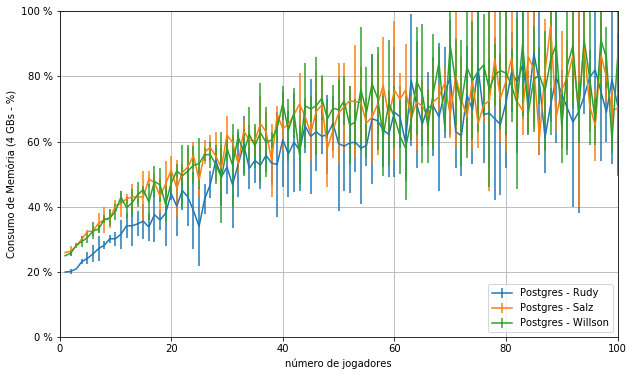
\includegraphics[width=0.8\textwidth]{figuras/analise/mem_db_media_por_jogador.png}
  \centering

  Fonte: O próprio autor.
\end{figure}

A partir da Figura~\ref{fig:mem_db_media_por_jogador} podemos confirmar as conclusões parciais obtidas da Tabela~\ref{tab:cpu_db_media_quadrantes}.
%
Além das conclusões parciais, é possível visualizar o crescimento da média a cada incremento de jogador simultâneo.
%
Podemos concluir que o serviço de fato foi estressado, haja vista que podemos perceber inicialmente um comportamento na qual não corresponde a uma curva multimodal.

A partir destes dados podemos concluir que:

$$
    MEM(db\_postgresql_{r}) < MEM(db\_postgresql_{s}) \approx MEM(db\_postgresql_{w})
$$

